\section{MATLAB implementation}

\subsection{The volatility surface in a stochastic volatility model}

\begin{par}
In this section we will compute prices and the implied volatility surface using the Heston model. The diffusion coefficient follows a stochastic process, which is correlated with the stock diffusion. This leads to a volatility smile or skew because one is able to recreate the leverage effect and a skewed return distribution like this. The dynamics of the Heston model are given by
\end{par} \vspace{1em}
\begin{par}
$$dS_t = \mu S_tdt + \sqrt{v_t}S_tdW_t^1$$
$$dv_t = \kappa (\theta - v_t)dt
+ \eta\sqrt{v_t}dW_t^2$$
\end{par} \vspace{1em}
\begin{par}
where $\langle W^1,W^2\rangle_t = \rho t$ and $\kappa , \theta , \eta , v_0 >0$.
\end{par} \vspace{1em}
\begin{par}
In this example we choose the model parameter as $v_0 = 0.2, \kappa = 0.5, \theta=0.2, \eta = 0.3\textrm{ and } \rho = -0.8$. Furthermore we are computing the values for a strike range from $60$ to $140$, a maturity range from $0.5$ to $3$, a underlying price of $100$ and a risk free interest rate of $5\%$. The divident yield is $0$ in this example.
\end{par} \vspace{1em}
\begin{verbatim}
model = 'HESTON';
paramsHeston = [.2,.5,.2,.3,-.8];
r=0.05; % risk free rate
S0=100; % underlying price
q=0; % dividend yield
n=40; %no. of strike steps

Tmin=0.5;
Tmax=3; %maximum value of time axis
Kmin=60;
Kmax=140; %maximum value of strike price axis

dt=(Tmax-Tmin)/(n-1);
T=(Tmin:dt:Tmax)';
dk=(Kmax-Kmin)/(n-1);
K=(Kmin:dk:Kmax)';
\end{verbatim}
\begin{par}
By using the function ImplVolSurf, we get the call prices and the corresponding volaility surface. This function calculates the prices by using the Lewis method, which is a Fourier transform pricing method.
\end{par} \vspace{1em}
\begin{verbatim}
[VolSurf, PriceSurface] = ImplVolSurf(S0, K, T, r, q, paramsHeston, model);
\end{verbatim}
\begin{par}
The following picture shows a surface plot of the computed volatility surface.
\end{par} \vspace{1em}
\begin{verbatim}
surf(K,T,VolSurf)
view([50.9000 33.2000])
title('An implied volatility surface')
ylabel('Maturity')
xlabel('Strike')
\end{verbatim}

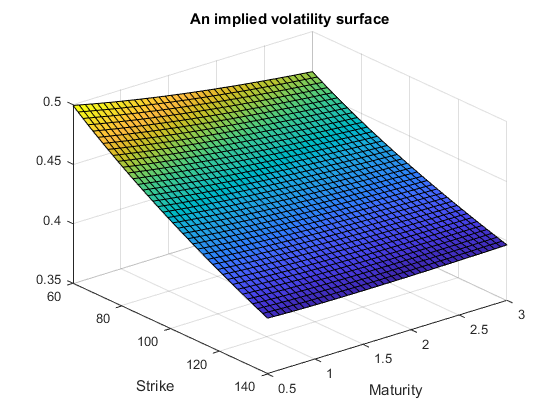
\includegraphics [width=4in]{fig/ScriptM_01.png}


\subsection{The local volatility surface}

\begin{par}
The goal of this section is to compute the local volatility by using the Dupire or BBF formula. We will use the output of the previous section.
\end{par} \vspace{1em}
\begin{par}
We can either compute the local volatility surface by using the prices and the Dupire formula or by using the implied volatility surface and the BBF formula. In this case we are using the Dupire formula. The function locVolSurf returns the local volatility surface, if we pass the input data (in our case the prices), the strike prices, the maturities, the risk free interest rate, the divident yield and a parameter which determines the used formula.
\end{par} \vspace{1em}
\begin{verbatim}
method = 'DUPIRE';
locVol = locVolSurf(K, T, r, q, PriceSurface, method, S0);
\end{verbatim}
\begin{par}
The following picture shows a surface plot of the computed local volatility surface.
\end{par} \vspace{1em}
\begin{verbatim}
surf(K(2:end-2),T(2:end-2),locVol)
view([50.9000 33.2000])
title('A local volatility surface')
ylabel('Maturity')
xlabel('Strike')
\end{verbatim}

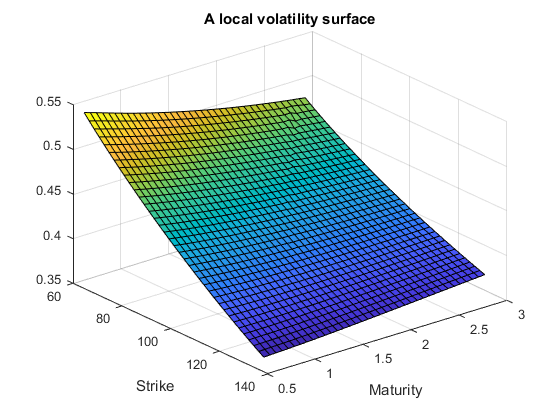
\includegraphics [width=4in]{fig/ScriptM_02.png}


\subsection{Practical use of the local volatility}

\begin{par}
Now we are going to use the local volatility in a Monte Carlo Euler simulator. In practice one can use the presented routine to price other, e.g. exotic derivatives. Our goal is to reprice the call options and to verify that the simulated call option prices match those we generated two sections ago (approximately). To simulate the price paths, we are going to use a modified version of the standard Euler scheme. We pass the local volatility surface, the other usual data and a parameter "Handle" to the function BSEulerMod. The Handle argument defines the action for the case when the simulated stock prices exceed the boundaries of the local volatility surface. If we pass TRUNC as Handle, the function will push the stocks prices back into the boundaries if the value of the simulated prices gets too big or too small. If we pass STOPS, the script will just ignore all the paths exceeding the boundaries.
\end{par} \vspace{1em}
\begin{verbatim}
Handle = 'NONE';
simN = 100000; % 100000 simulations
SimPrices = BSEulerMod(simN,dt,S0,K,T,r,q,locVol,Handle);
\end{verbatim}
\begin{par}
Now we compute the Call prices by using the CallPutPricer and compare the results to the original prices by calculating the relative error.
\end{par} \vspace{1em}
\begin{verbatim}
simPriceSurf = zeros(length(T)-3,length(K)-3);
for i = 3:length(T)-1
    for j = 2:length(K)-2
        simPriceSurf(i-2,j-1) = CallPutPricer(S0,...
        	SimPrices(:,i-1),K(j),T(i),r,q);
    end
end
RelError = abs(simPriceSurf-PriceSurface(3:length(T)-1,...
	2:length(K)-2))./PriceSurface(3:39,2:38);
\end{verbatim}
\begin{par}
The following picture shows the relative error of the simulated prices, computed without emergency stops and without truncation values.
\end{par} \vspace{1em}
\begin{verbatim}
surf(K(2:end-2),T(3:end-1),RelError)
title('Relative error')
ylabel('Maturity')
xlabel('Strike')
\end{verbatim}

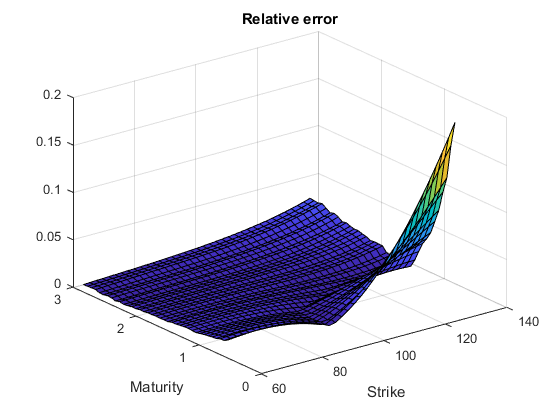
\includegraphics [width=4in]{fig/ScriptM_03.png}
\begin{par}
To see how emergency stops and truncation values effect the simulation, we plot the relative errors of all three methods into one figure.
\end{par} \vspace{1em}
\begin{verbatim}
surf(K(2:end-2),T(3:end-1),RelError)
title('Relative error comparison')
ylabel('Maturity')
xlabel('Strike')
hold

Handle = 'TRUNC';
SimPrices = BSEulerMod(simN,dt,S0,K,T,r,q,locVol,Handle);
simPriceSurf = zeros(length(T)-3,length(K)-3);
for i = 3:length(T)-1
    for j = 2:length(K)-2
        simPriceSurf(i-2,j-1) = CallPutPricer(S0,...
        	SimPrices(:,i-1),K(j),T(i),r,q);
    end
end
RelError = abs(simPriceSurf-PriceSurface(3:length(T)-1,...
	2:length(K)-2))./PriceSurface(3:39,2:38);
surf(K(2:end-2),T(3:end-1),RelError)

Handle = 'STOPS';
SimPrices = BSEulerMod(simN,dt,S0,K,T,r,q,locVol,Handle);
simPriceSurf = zeros(length(T)-3,length(K)-3);
for i = 3:length(T)-1
    for j = 2:length(K)-2
        simPriceSurf(i-2,j-1) = CallPutPricer(S0,...
        	SimPrices(:,i-1),K(j),T(i),r,q);
    end
end
RelError = abs(simPriceSurf-PriceSurface(3:length(T)-1,...
	2:length(K)-2))./PriceSurface(3:39,2:38);
surf(K(2:end-2),T(3:end-1),RelError)
hold off
legend('NONE','TRUNC','STOPS')
view([42.500 32.400])
\end{verbatim}
    
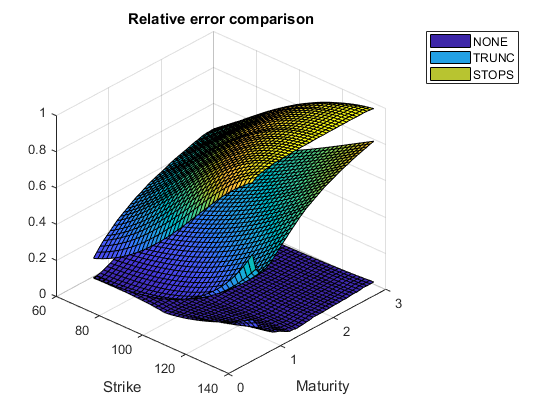
\includegraphics [width=4in]{fig/ScriptM_04.png}


\subsection{Implied volatility as "time-average" of the local volatility}

\begin{par}
As mentioned in a previous section, one can show that, under some technical conditions, the implied volatility is at large strikes approximately a time-average of the local volatility, i.g.
\end{par} \vspace{1em}
\begin{par}
$$I^2(t,x)=\frac{1}{t} \int_0^t (\sigma_u^\pm )^2du$$
\end{par} \vspace{1em}
\begin{par}
where $x(K,S) = \log\left(\frac{K}{S\exp\left(\mu t\right)}\right)$, $\sigma_t^\pm=\lim_{x\to\pm\infty}\sigma_t(x)$ and $I(t,x)$ denotes the implied volatility as a function of the log-forward-moneyness variable $x$.
\end{par} \vspace{1em}
\begin{par}
In this section we try to verify this formula. We do so by calculating the implied and local volatility for a high strikes and comparing both sides of the formula. We need to respecify the model parameter to meet the technical conditions and compute the new prices.
\end{par} \vspace{1em}
\begin{verbatim}
n=50;
T = (0.1:0.1:n*0.1)';
Kmin=60;
Kmax=150;
dk=(Kmax-Kmin)/(n-1);
K=(Kmin:dk:Kmax)';
paramsHeston = [0.05,0.5,0.2,0.001,-0.8];
[surface, PriceSurface] = ImplVolSurf(S0, K, T, r, q,...
	 paramsHeston, 'HESTON');
locSurf = locVolSurf(K,T,r,q,PriceSurface,'DUPIRE');
\end{verbatim}
\begin{par}
We approximate the integral by integrating numerically and we calculate a relative error like we did in the previous section.
\end{par} \vspace{1em}
\begin{verbatim}
integrand = locSurf(:,end).^2;
ImplVolAppr = ones(length(T)-4,1);
for i = 3:length(T)-2
    ImplVolAppr(i-2) = sqrt(1/T(i)*trapz(T(2:i),integrand(1:i-1)));
end
RelAppError = abs(ImplVolAppr-surface(3:length(T)-2,end-2))/...
	surface(3:length(T)-2,end-2);
\end{verbatim}
\begin{par}
The following image shows the relative error of the approximations with respect to the maturity.
\end{par} \vspace{1em}
\begin{verbatim}
plot(T(3:end-2),RelAppError)
title('Relative error')
xlabel('Maturity')
\end{verbatim}

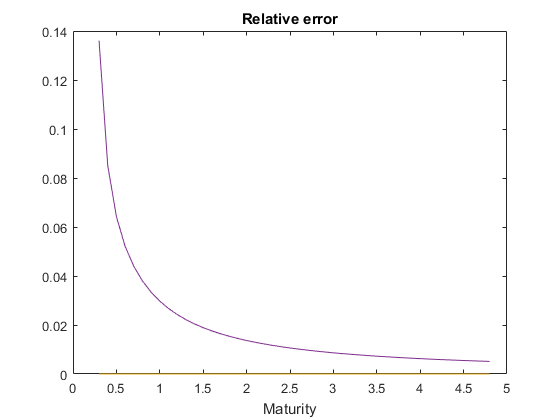
\includegraphics [width=4in]{fig/ScriptM_05.png}


\subsection{Implied volatility as "harmonic mean" of the local volatility}

\begin{par}
As allready mentioned, at very short maturity, the implied volatility at log-forward-moneyness $x$ is the harmonic mean of the local volatility across the moneyness dimension up to $x$, i.g.
\end{par} \vspace{1em}
\begin{par}
$$I^2(0,x) = \frac{x}{\int_0^x\frac{1}{\sigma_0^2(u)}du}.$$
\end{par} \vspace{1em}
\begin{par}
Now we proceed like we did in the previous section.
\end{par} \vspace{1em}
\begin{verbatim}
n=100; %no. of strike steps
T = (0.1:0.1:10*0.1)';
Kmin=100;
Kmax=130; %maximum value of strike price axis
dk=(Kmax-Kmin)/(n-1);
K=(Kmin:dk:Kmax)';

[surface, prices] = ImplVolSurf(S0, K, T, r, q,...
	 paramsHeston, 'HESTON');

locSurf = locVolSurf(K,T,r,q,prices,'DUPIRE');

integrand = 1./(locSurf(1,:).^2);
ImplVolAppr = zeros(length(K)-4,1);
for i = 3:length(K)-2
    ImplVolAppr(i-2) = sqrt(log(K(i)/S0)./(trapz(log(K(2:i)/S0),...
    	integrand(1:i-1))));
end
RelAppError = abs(ImplVolAppr-surface(2,3:length(K)-2))/...
	surface(2,3:length(K)-2);

plot(K(3:end-2),RelAppError)
title('Relative error')
xlabel('Strike')
\end{verbatim}

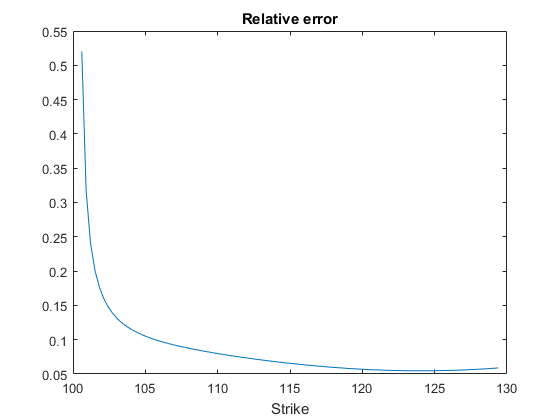
\includegraphics [width=4in]{fig/ScriptM_06.png}